\section{Trasformata di Fourier}
\lecture{4}{7 marzo 2024}

Nella soluzione generale abbiamo studiato esclusivamente funzioni periodiche con proprietà comode che sono spesso verificate nei sistemi fisici. Il secondo passo è studiare una funzione che descriva un effetto limitato nel tempo: possiamo immaginare che abbia un periodo \(T \to \infty \).

Consideriamo un intervallo di tempo ampio T tra \(-\frac{T}{2}\) e \(+\frac{T}{2}\) e risolviamo \(\hat{L} (x) = f(t)\). In questo intervallo, posso approssimare \(f(t)\) con una serie di Fourier detta \(f_s(t)\). Nell'intervallo, \(f_s(t)\to f(t)\). La serie di Fourier più comoda è la serie complessa.

\begin{figure}[H]
	\centering
	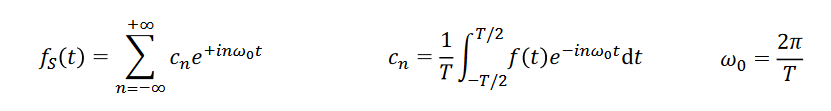
\includegraphics[width=0.8\textwidth]{2024-03-07-09-20-30.png}
	\caption{La serie scelta.}
\end{figure}

Mi limito a funzioni continue, integrabili e con \(\int_{-\infty}^{\infty} \vert f(t) \vert  \,\mathrm{d}t \) finito.

\begin{figure}[H]
	\centering
	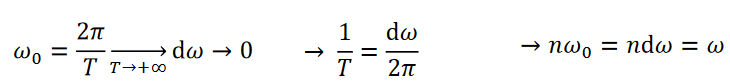
\includegraphics[width=0.8\textwidth]{2024-03-07-09-23-47.png}
	\caption{Gli elementi della serie diventano infinitesimi se \(T \to \infty \). }
\end{figure}

La pulsazione \(\omega \) è una variabile continua, anche se è data dal prodotto di un numero intero n e un infinitesimo \(\mathrm{d} \omega  \). Sto operando un passaggio dal discreto al continuo. 

\begin{figure}[H]
	\centering
	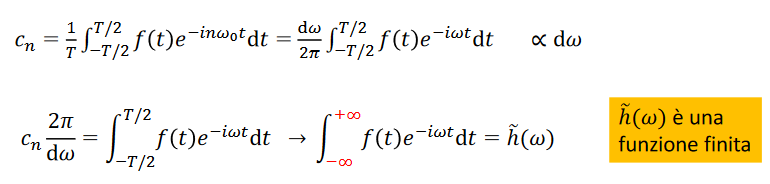
\includegraphics[width=0.8\textwidth]{2024-03-07-09-28-07.png}
	\caption{Divido per \(\mathrm{d}\omega  \) per evitare che il secondo membro tenda a zero. Il risultato è una funzione continua e finita, ottenuta integrando su tutti i tempi (\(T \to \infty \) ). }
\end{figure}

\begin{figure}[H]
	\centering
	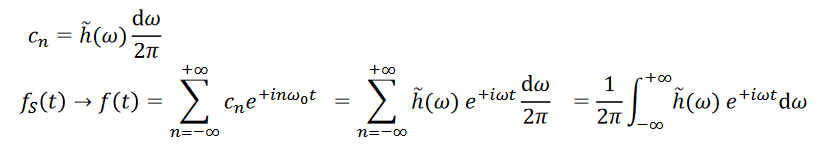
\includegraphics[width=0.8\textwidth]{2024-03-07-09-29-55.png}
	\caption{Adesso che ho una dipendenza da \(\mathrm{d}\omega  \) posso trasformare la sommatoria in un integrale. Rappresentando tutti gli n rappresento tutte le \(\omega \).  }
\end{figure}

\begin{definition}
	[Trasformata di Fourier]
	Data una funzione continua, a modulo integrabile, definita sull'asse reale, si definisce trasformata di Fourier della funzione f(t):
	\[
		\widetilde{f}(\omega )=\int_{-\infty}^{\infty} f(t)e^{i \omega t} \,\mathrm{d}t  
	\]
	\(\widetilde{f}(\omega ) \) descrive la componente di \(e^{i \omega t}\) nella funzione di partenza. La \(f(t)\) è rappresentabile come sovrapposizione continua di fasori:
	\begin{figure}[H]
		\centering
		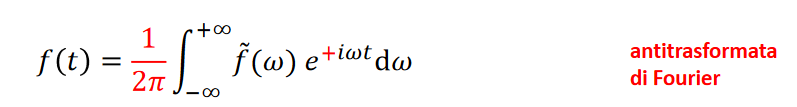
\includegraphics[width=0.8\textwidth]{2024-03-07-09-36-07.png}
		\caption{Antitrasformata di Fourier.}
	\end{figure}   
\end{definition}

La differenza con la serie di Fourier è che nella trasformata di Fourier siamo passati al continuo, mentre nella serie avevamo delle pulsazioni discrete. Questo procedimento è del tutto generale. Analizziamo le proprietà della trasformata di Fourier. Sia \(\mathcal{F} \) l'operatore trasformata di Fourier:

\begin{itemize}
	
	\item \(\mathcal{F} \) è lineare:
	\begin{figure}[H]
		\centering
		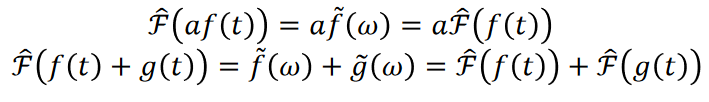
\includegraphics[width=0.8\textwidth]{2024-03-07-09-40-06.png}
		\caption{Proprietà dell'operatore \(\mathcal{F} \). }
	\end{figure}
	
	\item Le derivate diventano moltiplicazioni, come già visto con i fasori:
	\begin{figure}[H]
		\centering
		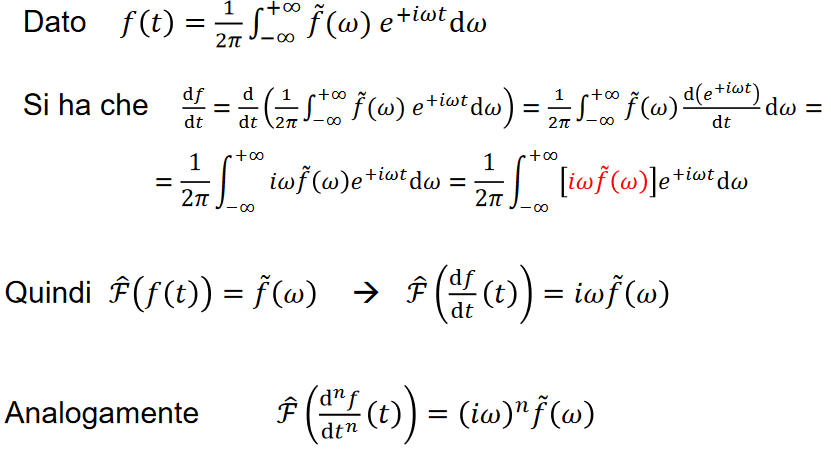
\includegraphics[width=0.8\textwidth]{2024-03-07-09-41-51.png}
		\caption{Alla terza riga ho l'espressione dell'antitrasformata della derivata di f, quindi il termine integrato corrisponde alla trasformata di Fourier.}
	\end{figure}
\end{itemize}

\subsection{Applicazione all'oscillatore armonico forzato}

Iniziamo applicando ad entrambi i membri della solita equazione la trasformata di Fourier.

\begin{figure}[H]
	\centering
	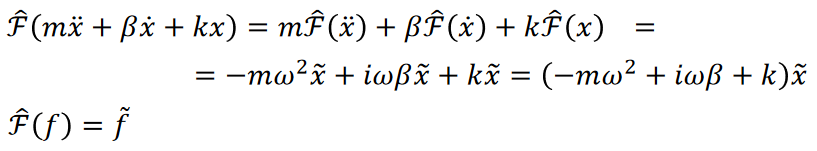
\includegraphics[width=0.8\textwidth]{2024-03-07-09-46-30.png}
	\caption{Ottengo così un'uguaglianza fra le due trasformate. Applico la seconda proprietà della trasformata di Fourier per cui le derivate diventano moltiplicazioni. \(\widetilde{x} \) è la mia incognita. }
\end{figure}

\begin{figure}[H]
	\centering
	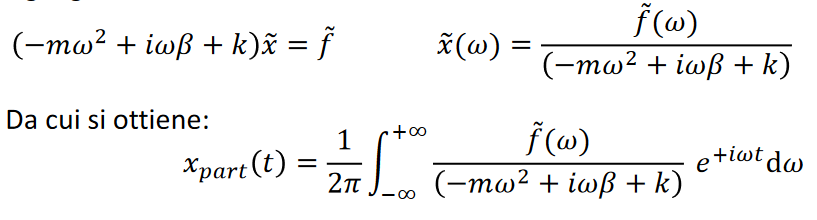
\includegraphics[width=0.8\textwidth]{2024-03-07-09-48-28.png}
	\caption{Così ho risolto il problema nello spazio delle pulsazioni. Con l'antitrasformata di Fourier posso trovare la soluzione particolare nello spazio dei tempi.}
\end{figure}

Non è chiaramente un processo matematico semplice, ma con l'aiuto dei computer questi integrali sono facilmente risolvibili numericamente. Proseguiamo con alcune osservazioni:
\begin{enumerate}
	
	\item Le equazioni differenziali lineari si trasformano in polinomi in \(\omega \):
	\begin{figure}[H]
		\centering
		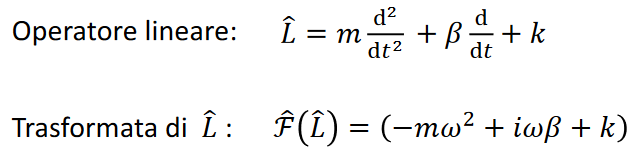
\includegraphics[width=0.8\textwidth]{2024-03-07-09-51-21.png}
		\caption{Posso vedere la trasformata di Fourier anche come un operatore che agisce su altri operatori.}
	\end{figure}
	
	\item t e \(\omega \) sono variabili coniugate. La trasformata di Fourier non è necessariamente collegata al tempo, basta avere due variabili coniugate: ad esempio, posso fare la trasformata di Fourier anche di un segnale periodico nello spazio. \(\frac{\mathrm{d}}{\mathrm{d}t} \leftrightarrow i \omega   \), il primo agisce nello spazio delle \(f(t)\) e il secondo agisce nello spazio delle \(\widetilde{f}(\omega ) \).  
\end{enumerate}

\begin{note}
	[Diverse definizioni di trasformata di Fourier]
	La definizione della trasformata di Fourier può essere diversa. Noi non le useremo mai! L'importante è associare l'antitrasformata corretta in base alla definizione di trasformata che abbiamo usato. Alcuni esempi:
	\begin{figure}[H]
		\centering
		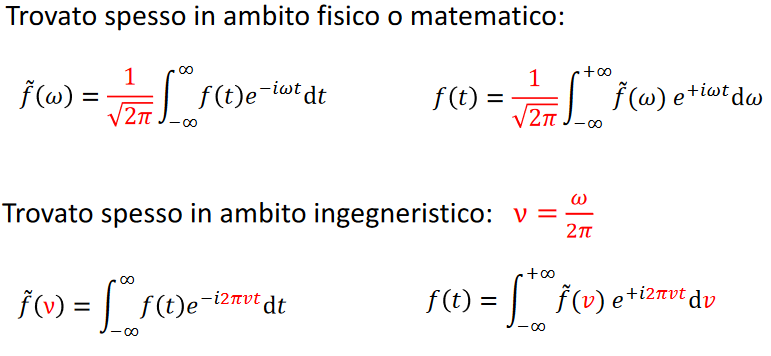
\includegraphics[width=0.8\textwidth]{2024-03-07-09-57-28.png}
		\caption{La prima è fatta per una questione di simmetria. La seconda è comoda per utilizzare il concetto di frequenza, che agli ingegneri sembra più naturale del concetto di pulsazione.}
	\end{figure}
\end{note}